\subsection{Background estimation of \texorpdfstring{\ttbar}{ttbar}}
Similar to the 8 \TeV analysis~\cite{Khachatryan:2016pup}, the estimation of the \ttbar background estimation is based on normalizing simulated templates in a $\mtll<100$ \GeV control region.
To render this simple technique feasible, we perform a number of cross-checks in order to assess the predictivity of the simulation of both, the \mtll shoulder and the tails.

%\subsubsection{Tails in  \texorpdfstring{\ttbar}{ttbar} and in \texorpdfstring{\ETmiss}{missing energy}}
We start by investigating the tails of the \ETmiss distribution and the different tail contributions of the \ttbar background in
both simulation and in data control regions.
First, we carefully scrutinize tail contributions in simulation and then we subsequently use data control regions to assess systematically large \ETmiss mismeasurements, the impact of lepton misidentifications and
the lepton fake rate.

\subsubsection{Disentangling the tail in \texorpdfstring{\mtll}{MT2ll} in simulated events. }
\label{sec:met_tail}
It is instructive to understand the various contributions that enter the simulated \mtll tail.
We perform the checks in the \texttt{MadGraph} sample which amounts to 300/fb, i.e. each event listed below enters with a weight of 0.03 for a data set of 10/fb.
The top quark and the W boson mass endpoints are exploited by the transverse mass variables \mtll, \mtlblb, \mtbb in both single-top and top-pair production and perfectly measured top quark events are expected to populate only the low regions of these variables. 
Moreover, semi-leptonic \ttbar events with a second fake or non-prompt lepton can not enter the \mtll tail. The reason is that \ETmiss satisfies the kinematical bound of $m_T(l_1,\ETmiss)<m_W$ because there is only one neutrino in the decay, and thus,
the hypothesis $p^{\nu 2}=0$ is a possible solution in the minimization procedure in the \mtll calculation. It follows that the kinematical endpoint is also respected by semileptonic \ttbar with
fake or non-prompt leptons. Consequently, not a single event from the 300/fb madgraph \ttbar sample that was generated in the semi-leptonic channel enters any of the signal regions in either {\verb Fall15 } or {\verb Spring16 } reconstruction. 

The remaining events in the tail fall into three broad categories. First, there are drastic mismeasurements of \ETmiss which are enough to promote
an event with two leptons to the \mtll tail. This can happen either by photons or neutral particles showering in e.g. a dead ECAL crystal or by a high energetic neutrino in a jet. Second, it can happen
that a lepton in a dileptonic \ttbar event does not pass reconstruction thresholds or ID requirements and a fake or non-prompt lepton is picked up instead.
In the latter category, the decay products of one of the W's may escape detection altogether and hence provide the source for extra \ETmiss.
Finally, there are events with hadronically decaying tau leptons which have extra genuine \ETmiss.

In order to understand the impact of less isolated leptons, we loosened the isolation requirement to $I_{\text{mini}}<0.2$ hand-scanned 38 simulated events in the search region $\mtll>140$ GeV
in {\verb Fall15 } samples. There were 5 events were found in the $\mu\mu$ channel, 11 in the $ee$ channel and 22 in the $e\mu$ channel.
The 19 events with mismeasured jets are distributed approximately independently of lepton flavor and 11 have highly energetic photons or pions showering in dead ECAL cells. 
One event in this category have two jets mismeasured.
We traced the generated particles individually and correlated their disappearance with known cracks in the detector. It is noteworthy, that the current simulation (Spring16)
correctly simulates all calorimetry dead cells. The remaining 8 events each had a neutrino produced inside a jet in excess of 40 GeV which is enough to promote the event to the tail. 
We checked that by treating the neutrino momentum as visible energy, the value for \mtll is in  the bulk of the \mtll distribution. In one extreme case, a 1.6 \TeV b-jet produced a 200 \GeV neutrino.
Another source is due to either lost electron (muon) or a hadronically decaying  tau lepton from one of the W-bosons combined with a non-prompt or fake lepton passing the lepton selections.
In such events a lepton from a W and a fake lepton are used to compute the \mtll and the resulting value does not respect to the W transverse mass endpoint anymore. 
There were 12 events involving a $\tau$ lepton of which 3 decayed leptonically. An overview of the situation from gen-level (top) to reco-level (bottom) is given in Fig.~\ref{fig:ttbar_tail}.

The study was repeated in {\verb Spring16 } with the nominal isolation requirement showing a reduction of the fake and non-prompt lepton component and compatible results on the \ETmiss related backgrounds. Results on event by event basis are listed in Tab.~\ref{tab:80Xtail}. 
\begin{table}
  \center
  \small
  \begin{tabular}{l|l|l}
  & event:run:lumi & result \\ 
  \hline 
0  &  1:4953:3991364    & gamma lost in dead cell (jet mism.)\\
1  &  1:5468:4532888    & jet mismeasurement at $\eta/\phi=$ -0.934/2.9678\\
2  &  1:6024:4854452    & $\gamma$ lost at $\eta/\phi=$ 1.6/-2.4, 1.9/2.7 small jet mism., $\nu$ from jet\\
3  &  1:6171:4972344    & jet mismeasurement (Ecal), 160 \GeV \\
4  &  1:12852:10356846  & lost $K^{+}$ at $\eta/\phi=$ 1.391/-2.527\\
5  &  1:13923:11219847  & looks like jet mismeasurement, no AOD available\\
6  &  1:17046:13736425  & gaussian jet mism., $\nu$ in jet \\
7  &  1:18692:15495640  & 40\GeV overmeasured $\mu$ at $\eta/\phi=$ 2.287/-0.282, jet mism.\\
8  &  1:20840:17276057  & lost high pt $\gamma$ at $\eta/\phi=$ -1.5/0.6 (jet mism.), $\nu$ in jet\\
9  &  1:25322:20991689  & $\nu$ in a jet of 100\GeV, just passing the threshold (142\GeV)\\
11 &  1:27005:21762195  & lost $\gamma$ and neutrals in dead cell $\eta/\phi=$ 1.152/-3.077 (jet mism.)\\
12 &  1:40541:33607796  & lost $\mu^-$ from W, picked up $e^-$ fake, \\&&some trk inefficieny at $\eta/\phi=$ -2.175/0.183 (seems gaussian)\\
13 &  1:48624:40308549  & lost high pt $\gamma$ (jet mism.)\\
14 &  1:49599:41117351  & lost mu- in a jet $\eta/\phi=$-0.999/0.558 \\
15 &  1:51330:42552044  & lost energy in ECAL (jet mism.) $\eta/\phi=$-0.837/2.890\\
16 &  1:57932:48024871  & fake $\mu$ at $\eta/\phi=$ 0.289/-2.763, also gaussian jet mismeasurement \\
17 &  1:62587:51884514  & jet mism. in a 200\GeV genjet, $\nu$ in another jet\\
18 &  1:65097:53964677  & lost $\mu$ to pt cut, picked up fake e from conversion $\gamma$,\\&& plus jet mism. (gaussian) \\
19 &  1:67998:56369604  & $\nu$ from jet\\
20 &  1:68445:56740873  & $\tau$ decaying hadronically, non-prompt $\mu$\\
21 &  1:71016:58872109  & fake $\mu$ with 60 \GeV inconsistency btw inner track and global track\\
22 &  1:72622:60203349  & $\nu$ in jet, several $\gamma$ lost in jet\\
23 &  1:74317:61608051  & 30 \GeV $\mu$ mism. at $\eta/\phi=$-2.275/-1.514\\
24 &  1:82880:68707320  & likely non-prompt $\mu$, no AOD available\\
25 &  1:85837:71158655  & $\nu$ from jet\\
26 &  1:94223:78110867  & $\gamma$ lost in crack\\
27 &  1:106121:87973932 & several mism. jets\\
28 &  1:113723:94275792 & jet mismeasurement at $\eta$ approx. 3, $\nu$ in a jet
  \end{tabular}
  \caption{Result of the tail scan of \ttbar in \texttt{Spring16} simulation.}
  \label{tab:80Xtail}
\end{table}


\begin{figure}[!hbtp]
\centering
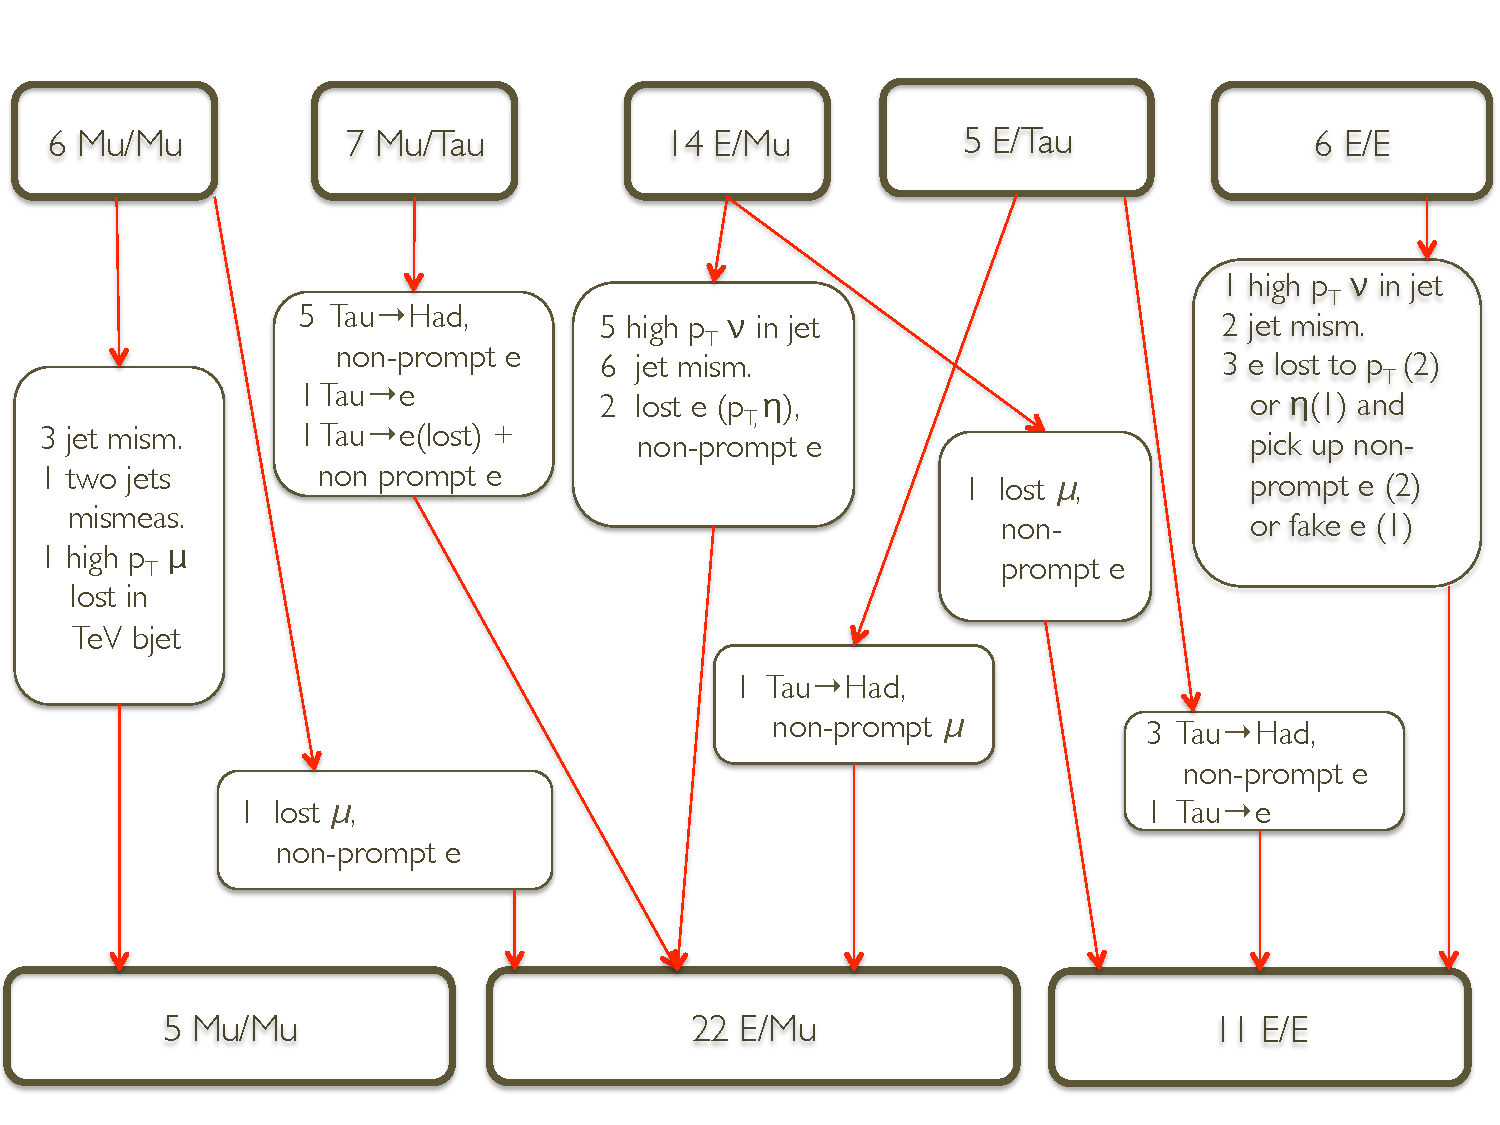
\includegraphics[width=0.9\textwidth]{figures/ttBar/ttbar_tail.pdf}
\caption{Overview of 38 events passing $\mt2ll>140$ GeV. Gen-level is at the top, reco-level at the bottom.}
\label{fig:ttbar_tail}
\end{figure}

Data control regions are formed to validate MC simulation for these sources and results are presented in the following sections.

\subsubsection{ Check of \ETmiss tails in DY data }

\begin{figure}[!hbtp]
\centering
\subfloat[]{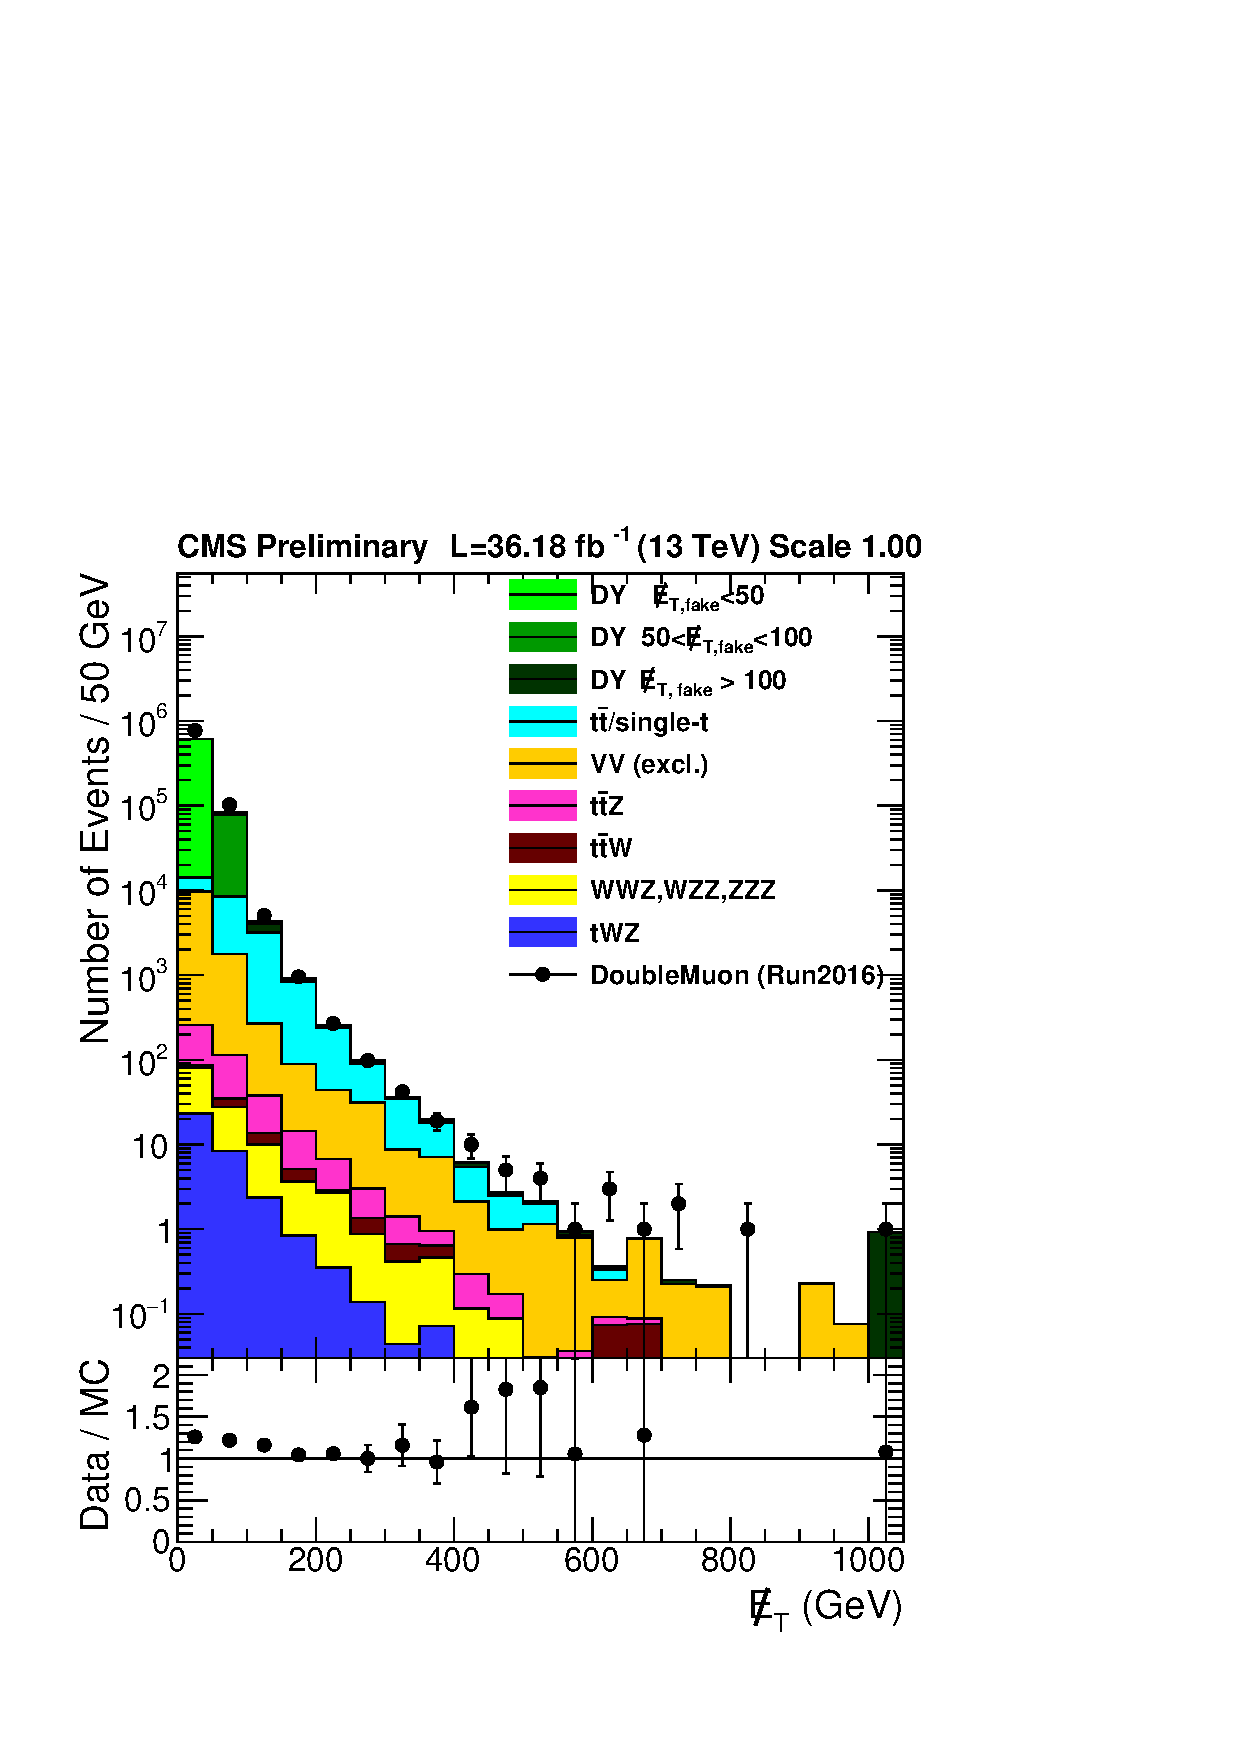
\includegraphics[scale=0.45]{figures/ttBar/met_control_met_pt_v2.pdf}}
\subfloat[]{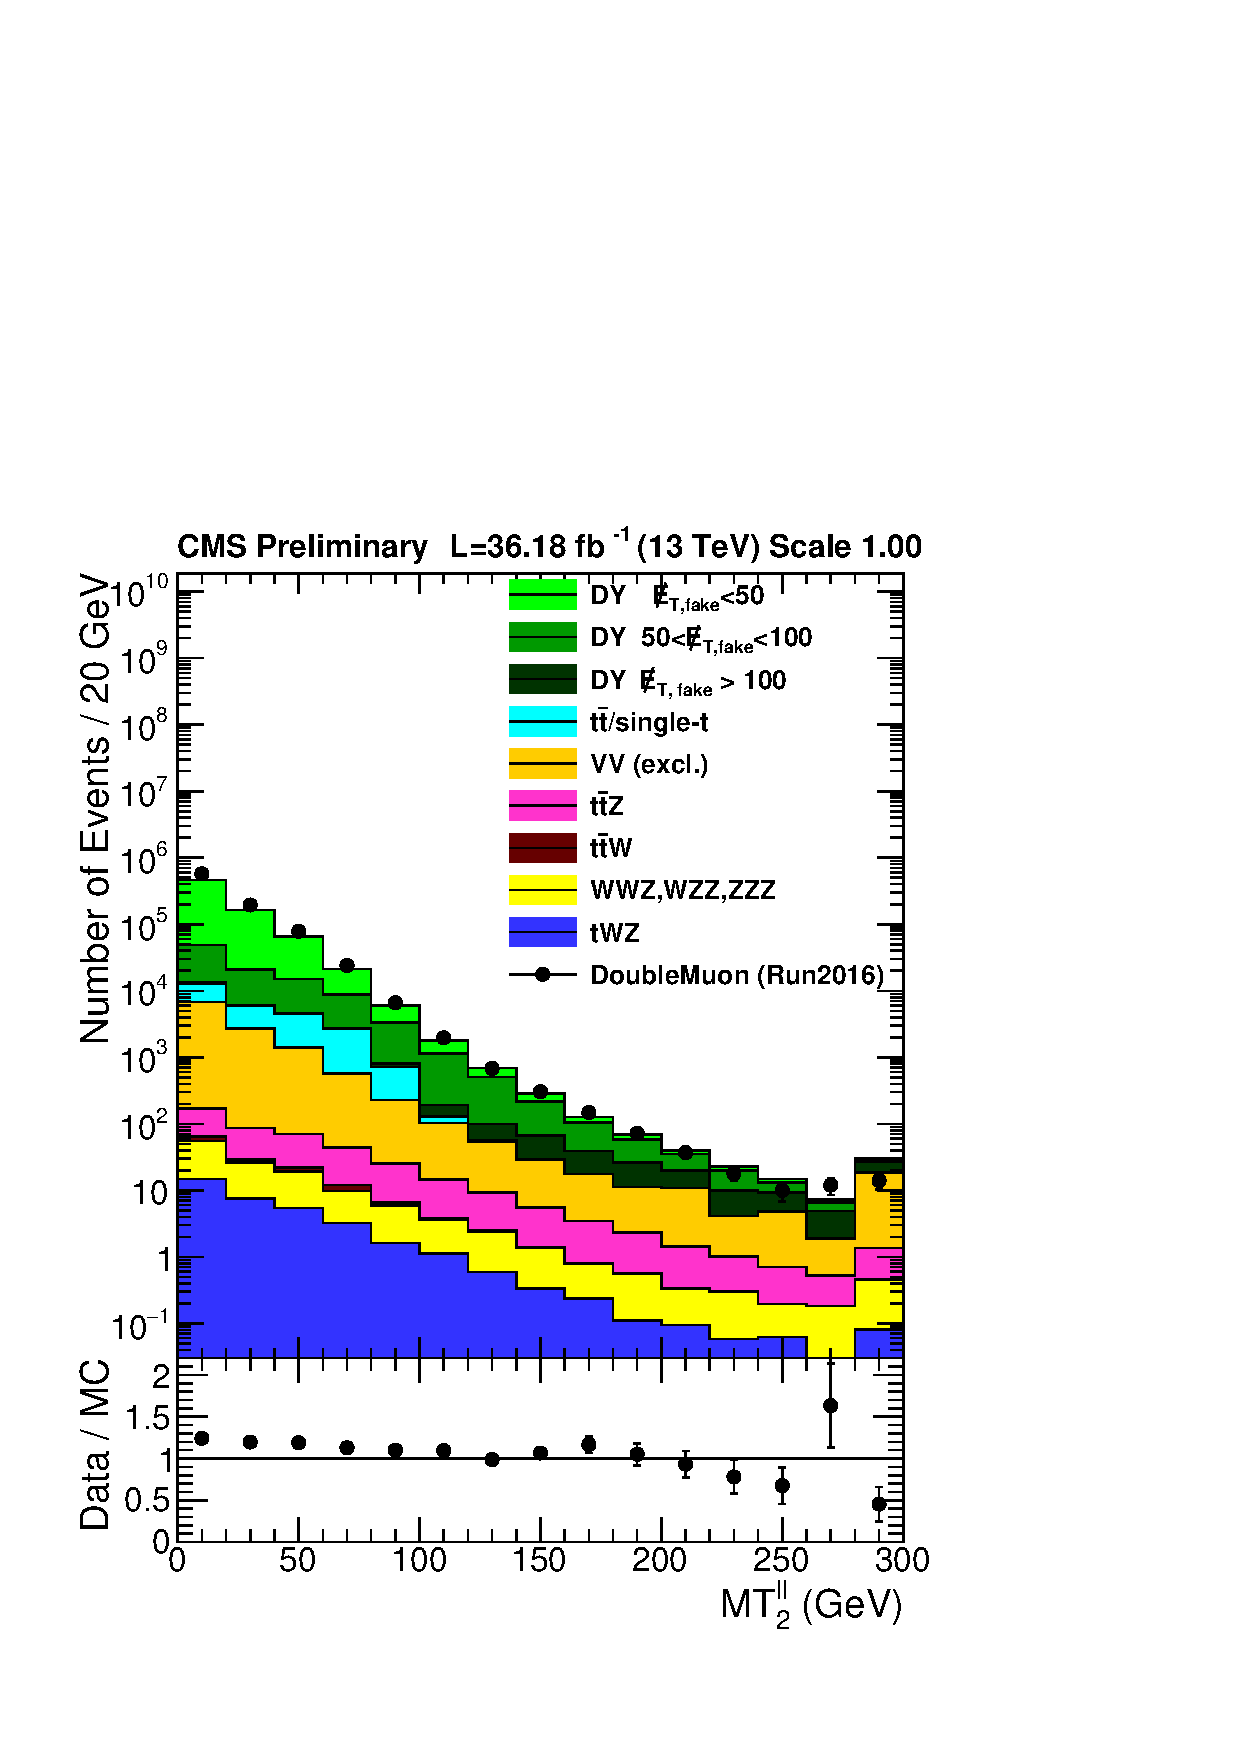
\includegraphics[scale=0.45]{figures/ttBar/met_control_dl_mt2ll_v2.pdf}}
\caption{ \ETmiss and \mtll distribution in the on-Z selection with 0 b-tags.}
\label{fig:met_tail_controlPlots}
\end{figure}

We proceed to check whether there is a sign of a higher rate of drastic jet mismeasurements in data. We can do that again in the 0 b-tag on-Z region selecting events
with zero genuine \ETmiss. The \ETmiss distribution is shown in Fig.\ref{fig:met_tail_controlPlots}a and the high \ETmiss tail is populated by \ttbar which, on the contrary, does predict genuine 
\ETmiss. In order to perform a sensible check anyways, we first split the DY sample in three bins of fake \ETmiss at thresholds of 50 \GeV and 100 \GeV shown in different shades of green.
Then, we exploit the excellent suppression of \mtll of dileptonic ttbar. The \mtll distribution is shown in Fig.\ref{fig:met_tail_controlPlots}b and shows that for $\mtll>100 \GeV$ the 
data is dominated by DY with large mismeasurements and that apparently there is no significant excess of events with jet mismeasurements.

\subsubsection{ Shape analysis of fake lepton backgrounds }

\begin{figure}[!hbtp]
\centering
\subfloat[Three-lepton control region]{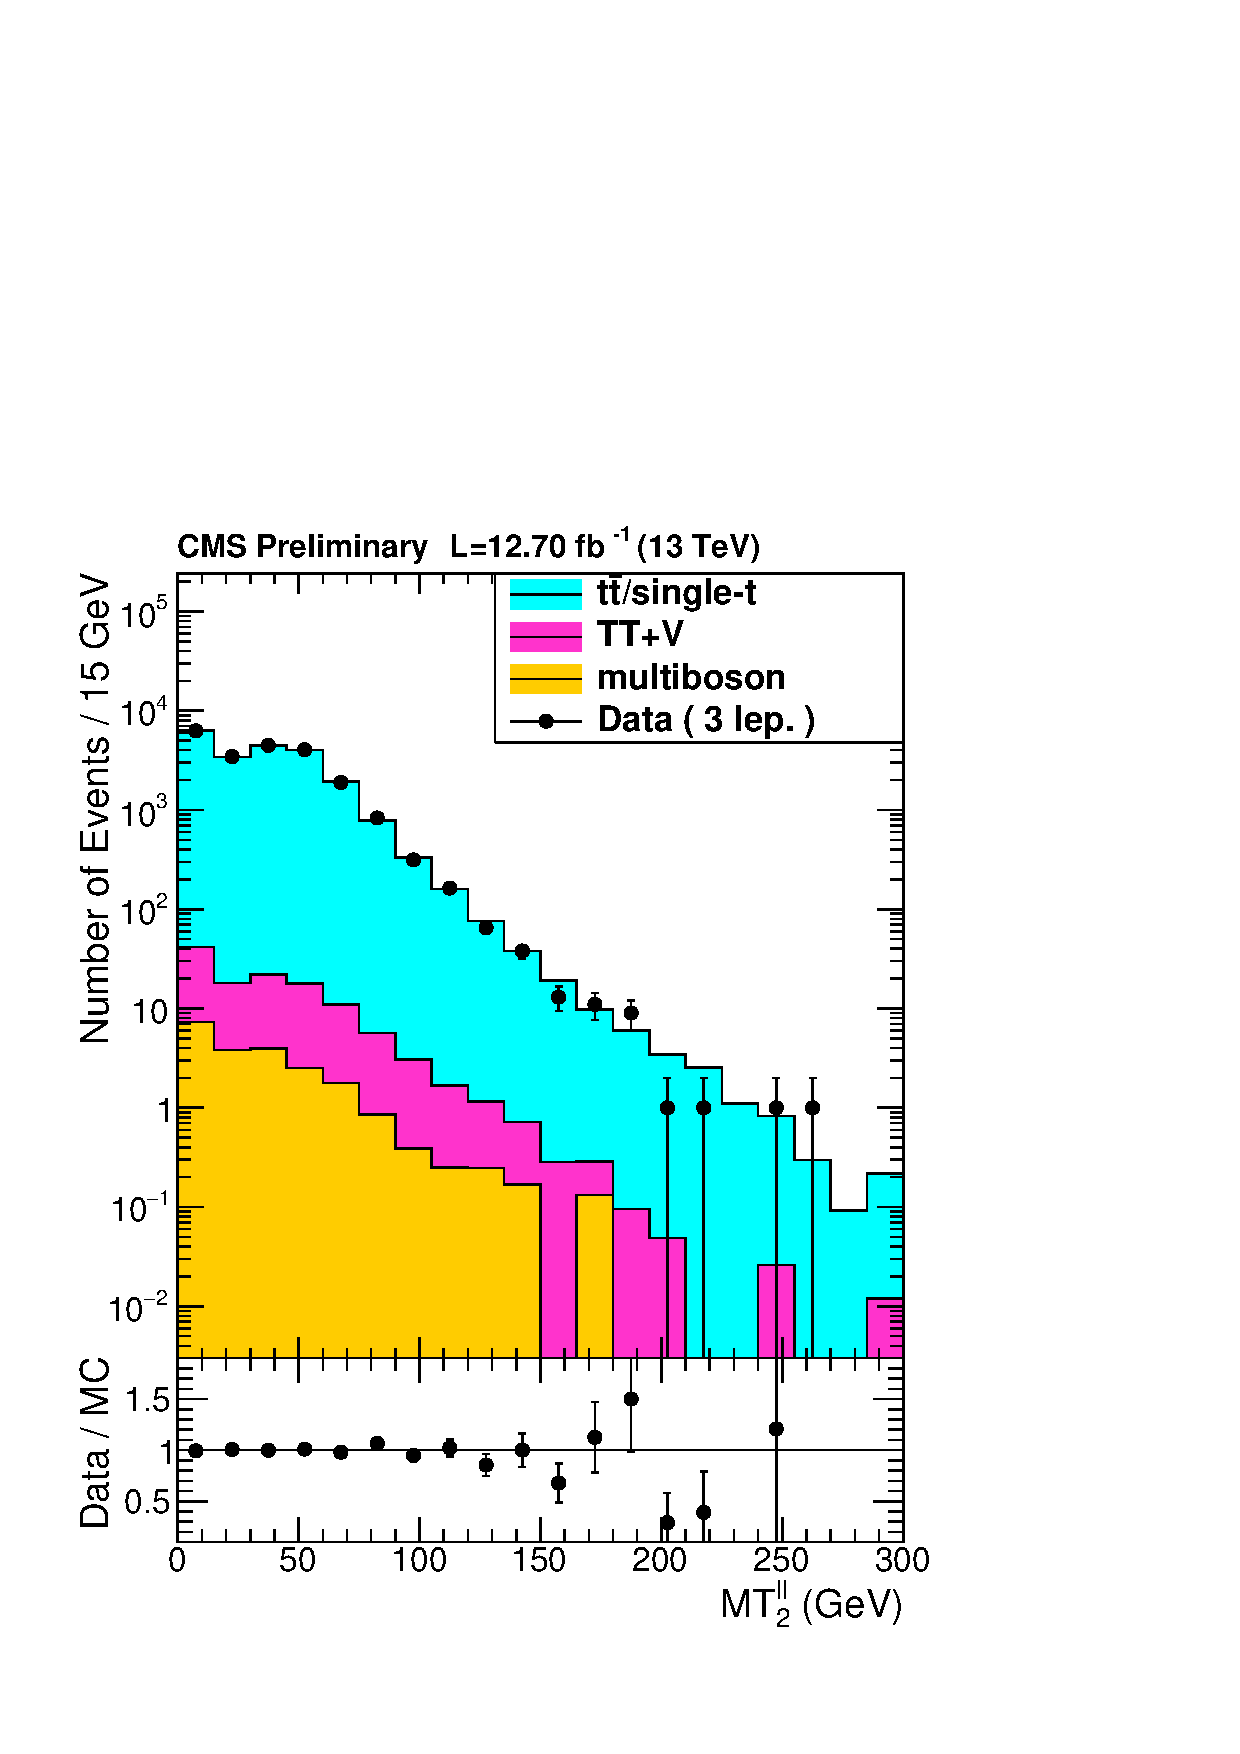
\includegraphics[width=0.35\textwidth]{figures/ttBar/all_dl_mt2ll.pdf}}
\subfloat[\ttbar 2l vs. 3l]{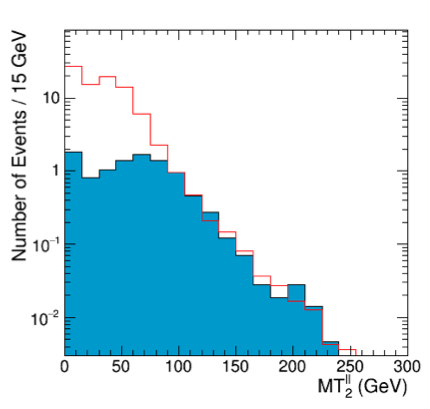
\includegraphics[width=0.5\textwidth]{figures/ttBar/MC_fake_shape_comparison.png}}
\caption{Left: \mtll distributions in two control regions enriched by $t\bar{t}$ events. MC yields are normalized to data using the yields at $\mtll<100$ \GeV. Right: Comparison of the three lepton simulation (blue area) 
and the two-lepton simulation with inverted isolation requirements on one lepton (red line), normalized at $\mtll>100$~\GeV. \FIXME{Robert, please update.}}
\label{fig:ttBar_3l}
\end{figure}

Next, we check whether the \mtll shape is correctly simulated. To this wend, we mimic lepton mis-identification by selecting three lepton events where the third lepton is selected with very loose requirements. 
%All other selections summarised in Table ~\ref{Tab:baselineSel} are applied. 
In order to imitate the loss of a lepton, we recompute \mtll by combining either the leading or the sub-leading lepton with the extra trailing lepton selected in this way.
We keep track of the changes in flavor channel associated with the lepton replacement.
This swapping procedure is applied to lepton momenta only, the \ETmiss is not changed because of the very high detection efficiency and compensating nature of the nearly hermetic CMS detector.
The procedure can be applied to both data and simulation and the resulting \mtll distribution is shown in Figure~\ref{fig:ttBar_3l}a and exhibits excellent agreement between data and simulation.

It remains to be shown that the swapping procedure really mimics the lost lepton contribution. This is done in Figure~\ref{fig:ttBar_3l}b where we overlay the two-lepton simulation with an inverted
isolation requirement $I_{\text{mini}}>0.2$ on the trailing lepton (red line) with the three-lepton prediction from the swapping procedure (blue area). 
The distributions are normalized for $\mtll>100$~\GeV and the almost perfect agreement confirms that the swapping procedure mimics the loss of a lepton very well for $\mtll>80$~\GeV. 
It should be noted that the swapping
procedure is not strongly dependent on the details of the selection of the extra leptons. As long as the loose selection guarantees that extra leptons are dominated by non-prompt decays in b-jets,
the reconstructed value of \mtll is governed by the relative angular position of the extra lepton and less by it's transverse momentum which is typically too small to have a very large effect.
We conclude that there are no signs of a discrepancy in the \mtll shape for events with a lost lepton.

\subsubsection{ Check of the lepton fake rate }
In order to verify that also the rate of fake leptons that enter in our selection is well modeled by MC we selected 3-lepton events where the two of the leptons are selected with tight requirements (same as in the analysis) and the 3${}^{\text{rd.}}$ lepton with a transverse momentum threshold of 10 GeV and relaxed isolation requirement. 
In addition, we ask $\Njets\geq2$ and $\Nbtags\geq1$ to select a similar phase space. No \ETmiss or \metSig requirements made. In this selection we check the distribution of $I_{\text{rel.mini}}$ and the standard relative isolation $I_{\text{rel}}$. 

\begin{figure}[!hbtp]
\centering
\subfloat[ $\mu\mu\mu$ ]{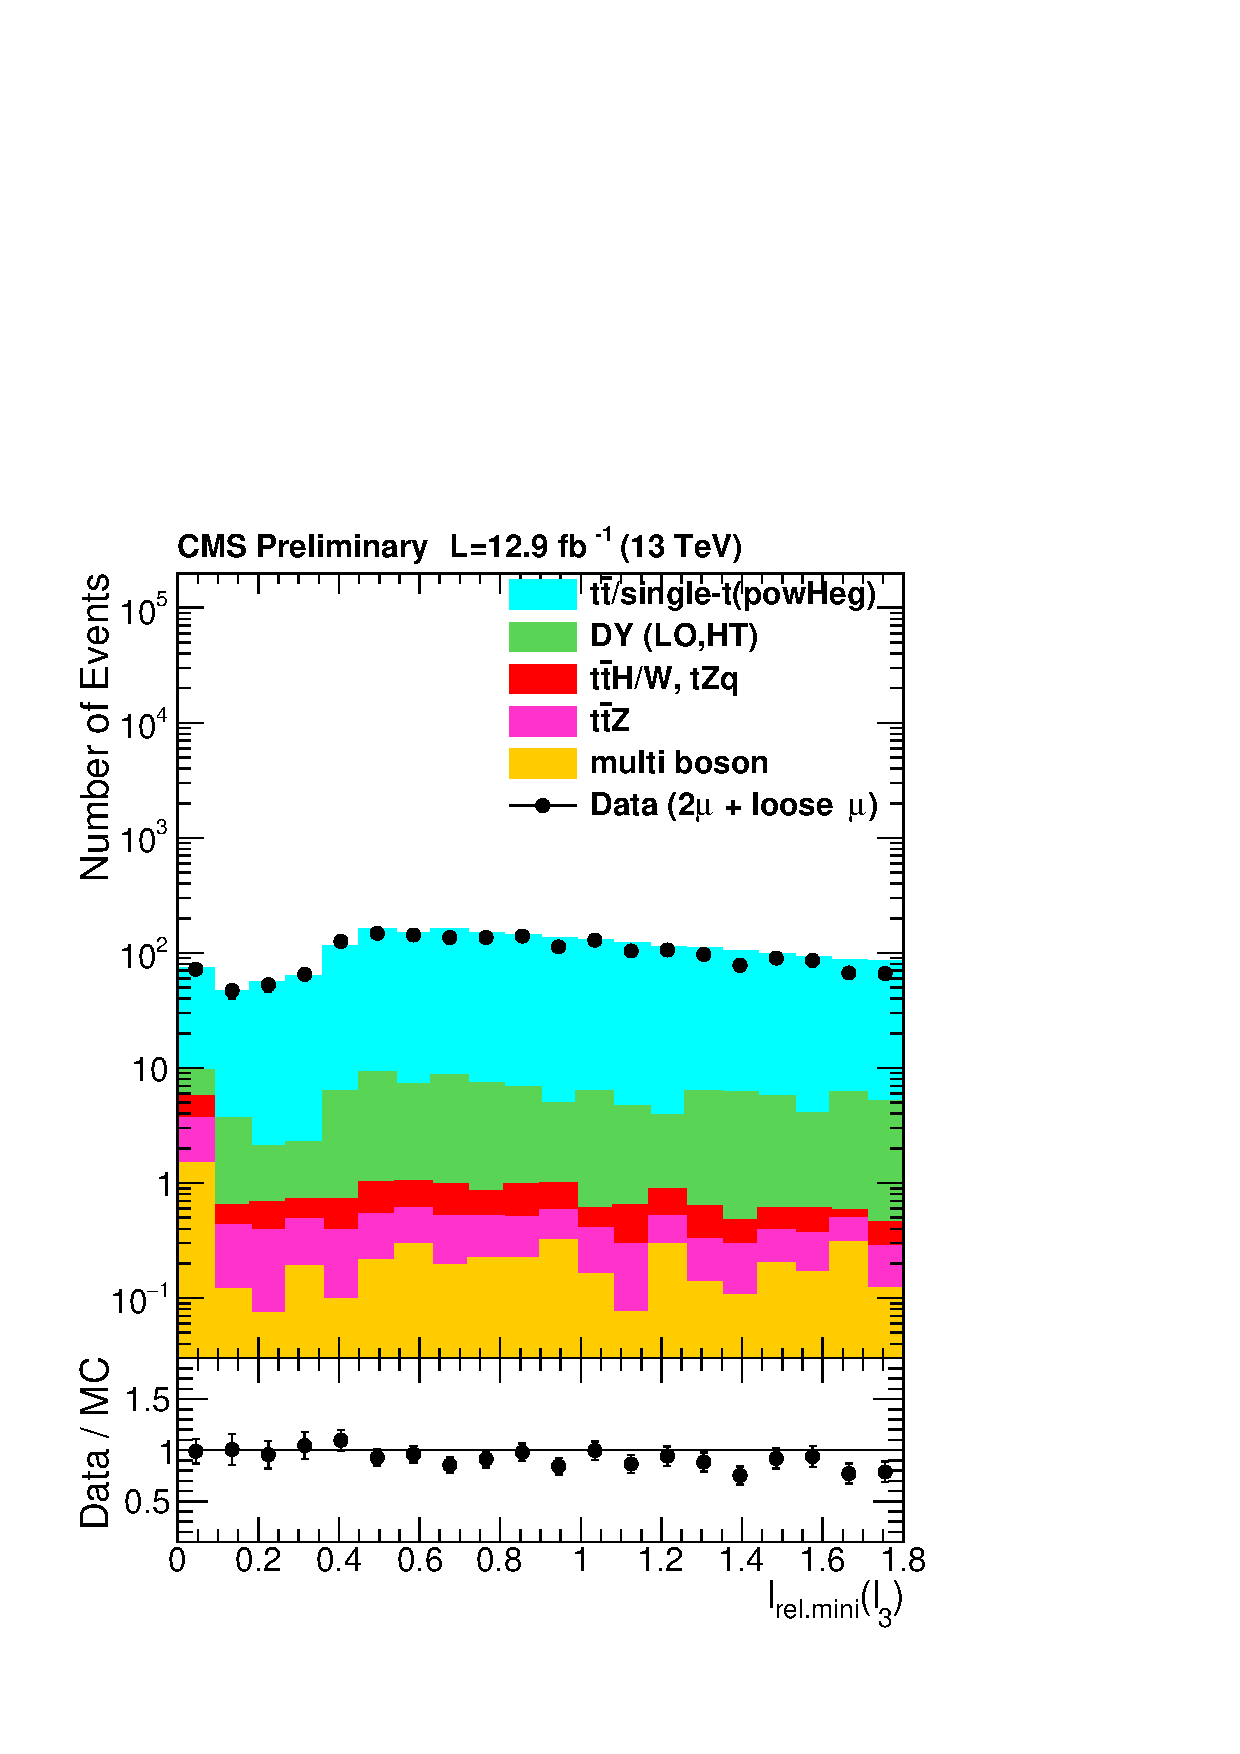
\includegraphics[scale=0.45]{figures/fakeRate/mumu_loose_mu_log/njet2-btagM-multiIsoWP/l3_miniRelIso.pdf}}
\subfloat[ eee ]{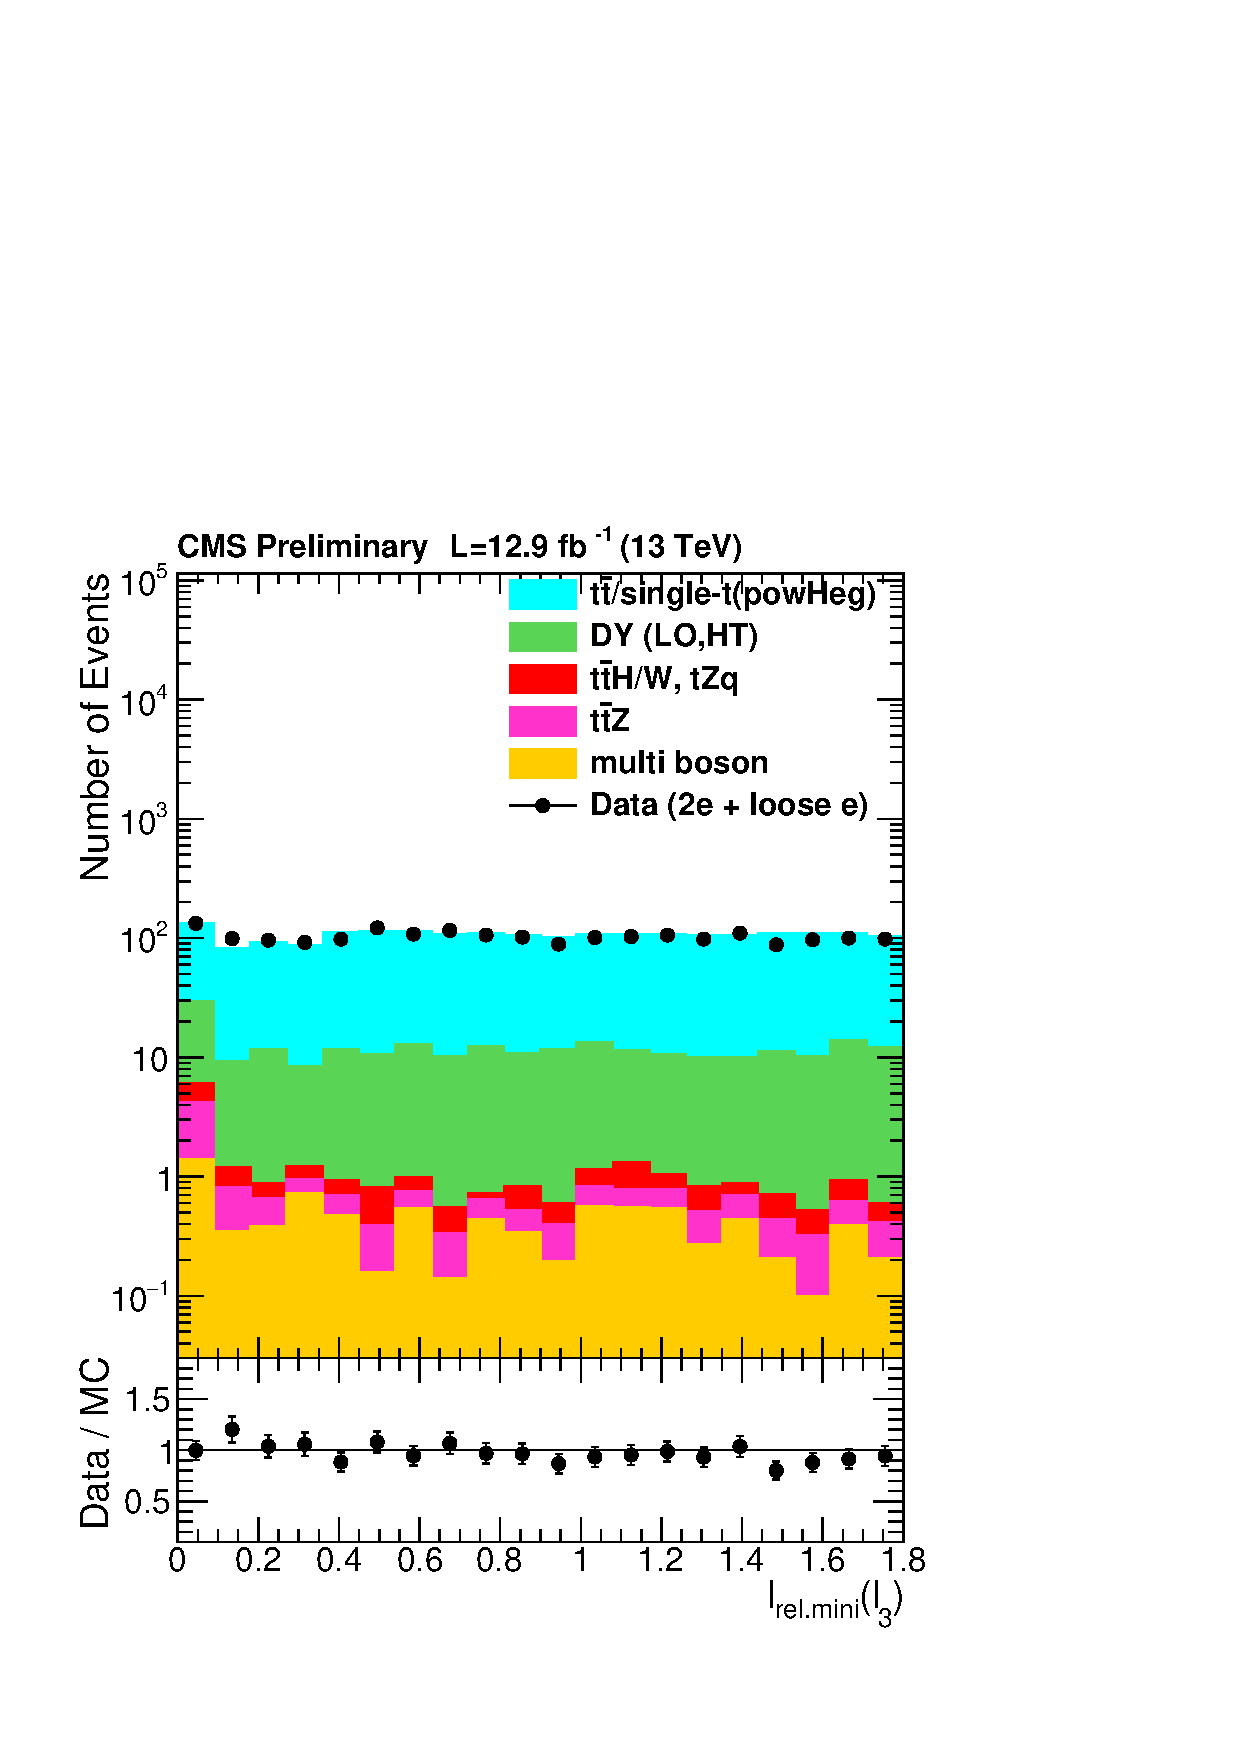
\includegraphics[scale=0.45]{figures/fakeRate/ee_loose_e_log/njet2-btagM-multiIsoWP/l3_miniRelIso.pdf}}
\caption{ $I_{\text{rel.mini}}$ and $I_{\text{rel.}}$ distribution of the third non-isolated lepton in the $\mu\mu\mu$ (left) and eee (right) channels. \FIXME{Tom, please update.}}
\label{fig:ttBar_FR_controlPlots}
\end{figure}

The distributions in Fig.\ref{fig:ttBar_FR_controlPlots} are normalized to luminosity. 
The fake-rate can be derived from the ratio of the first bin to the rest of the distribution. 
From the reasonably good agreement between data and simulation for the shape of the distributions, we conclude that the FR in data matches the one in MC. 
Nonetheless, we deduce an 15\% uncertainty driven by the available statistics in the first bins.

\subsubsection{ Validating the \texorpdfstring{\ttbar}{ttbar} shape in control regions at high and low \ETmiss}

\begin{figure}[!hbtp]
\centering
\subfloat[ $\Njets \leq 1$, $\Nbtags=0$, high \ETmiss]{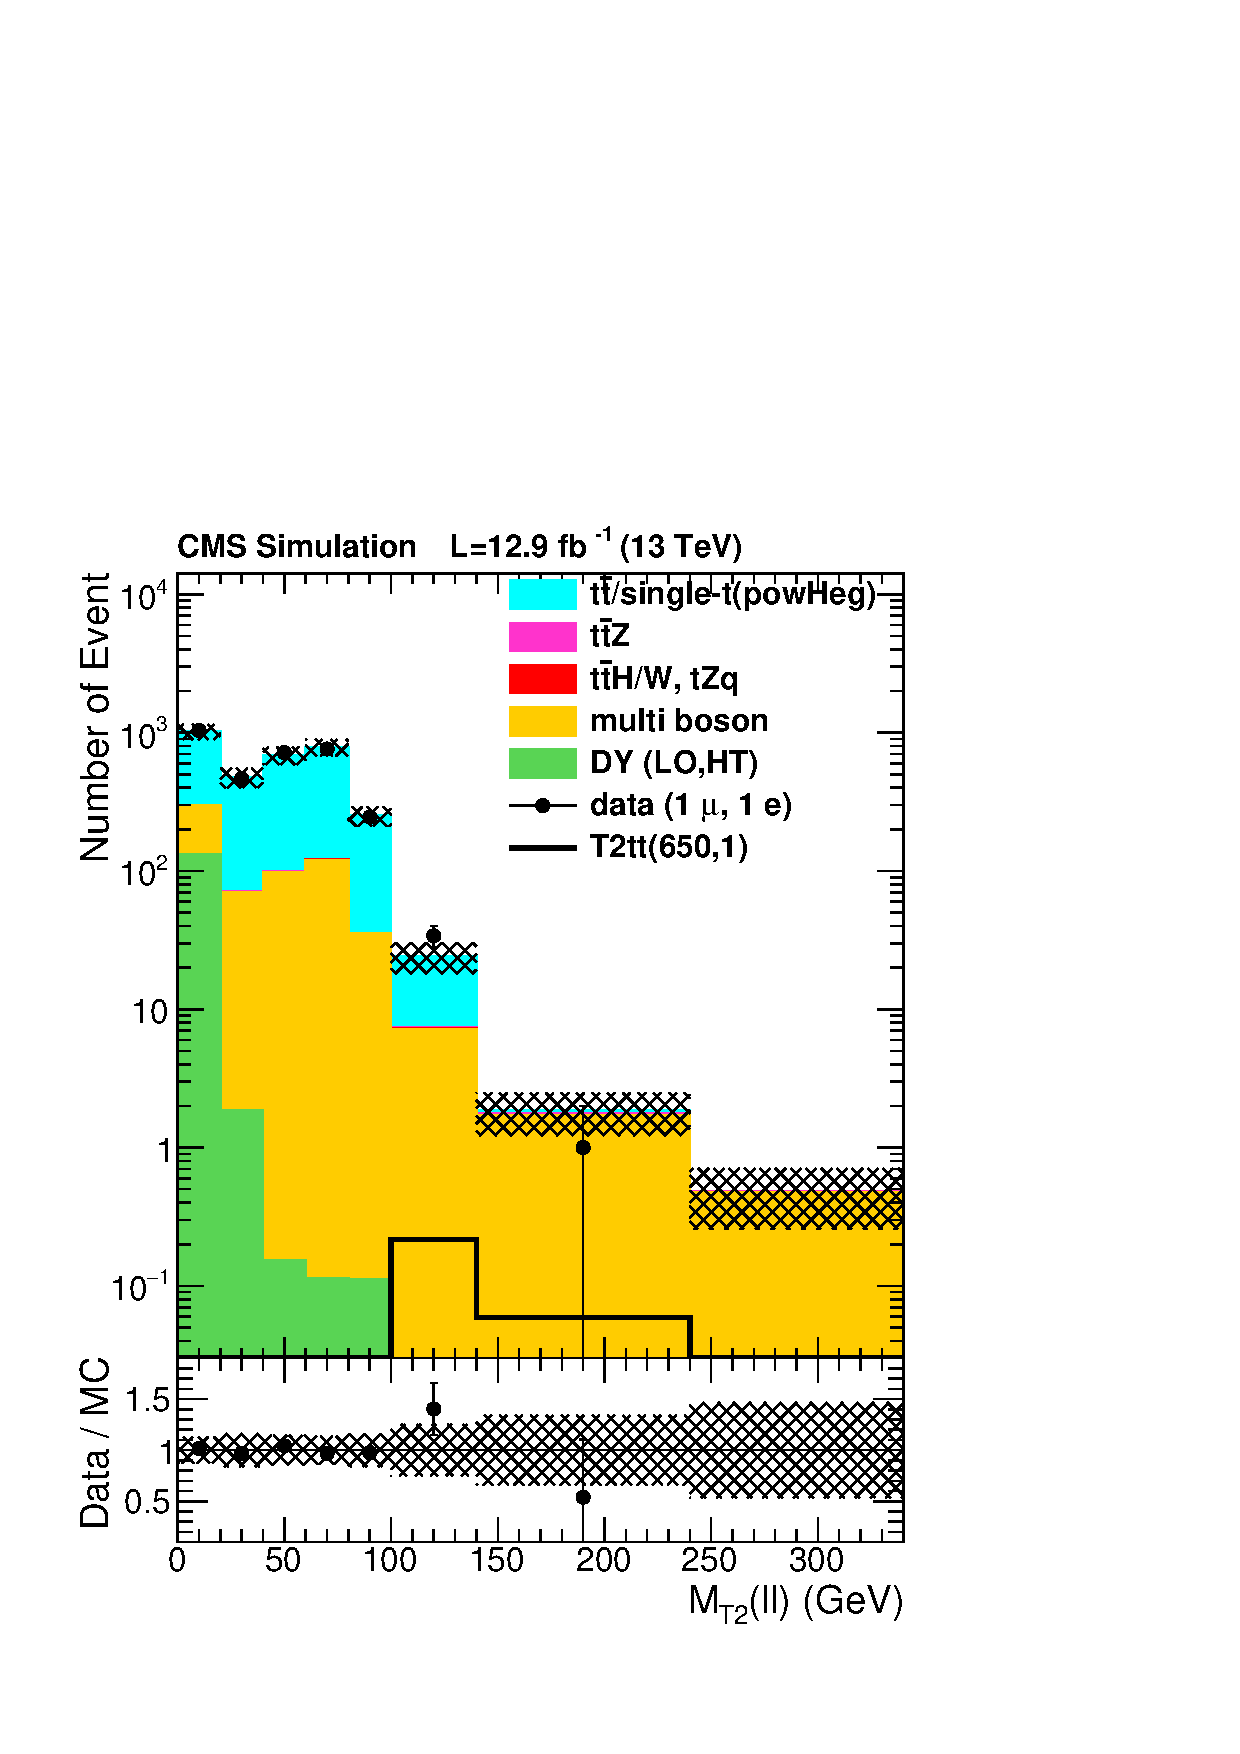
\includegraphics[scale=0.33]{figures/systematicPlots/mue_log_scaled/njet01-btag0-multiIsoWP-looseLeptonVeto-mll20-met80-metSig5/dl_mt2ll.pdf}}
\subfloat[ $\Njets \leq 1$, $\Nbtags\geq1$, high \ETmiss]{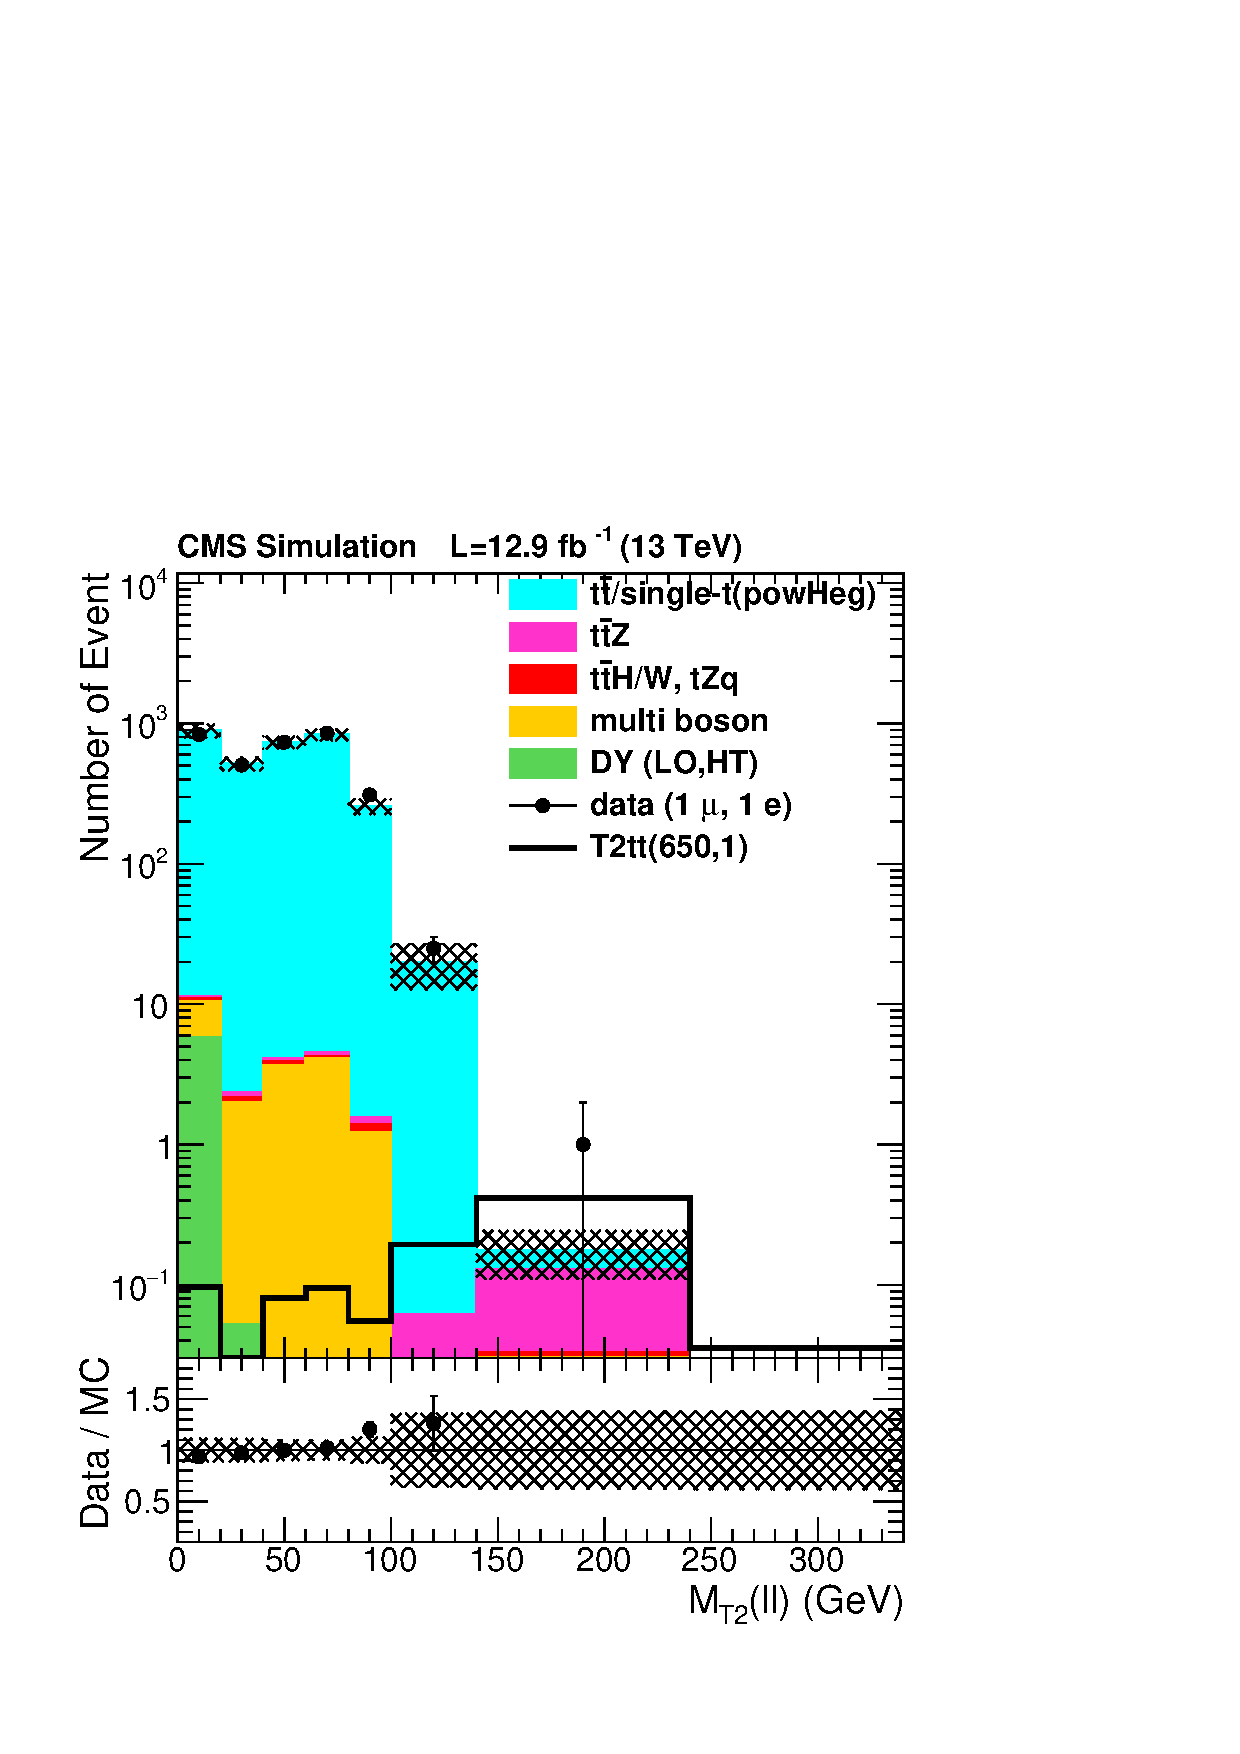
\includegraphics[scale=0.33]{figures/systematicPlots/mue_log_scaled/njet01-btagM-multiIsoWP-looseLeptonVeto-mll20-met80-metSig5/dl_mt2ll.pdf}}
\subfloat[ $\Njets \geq 2$, $\Nbtags=0$, high \ETmiss]{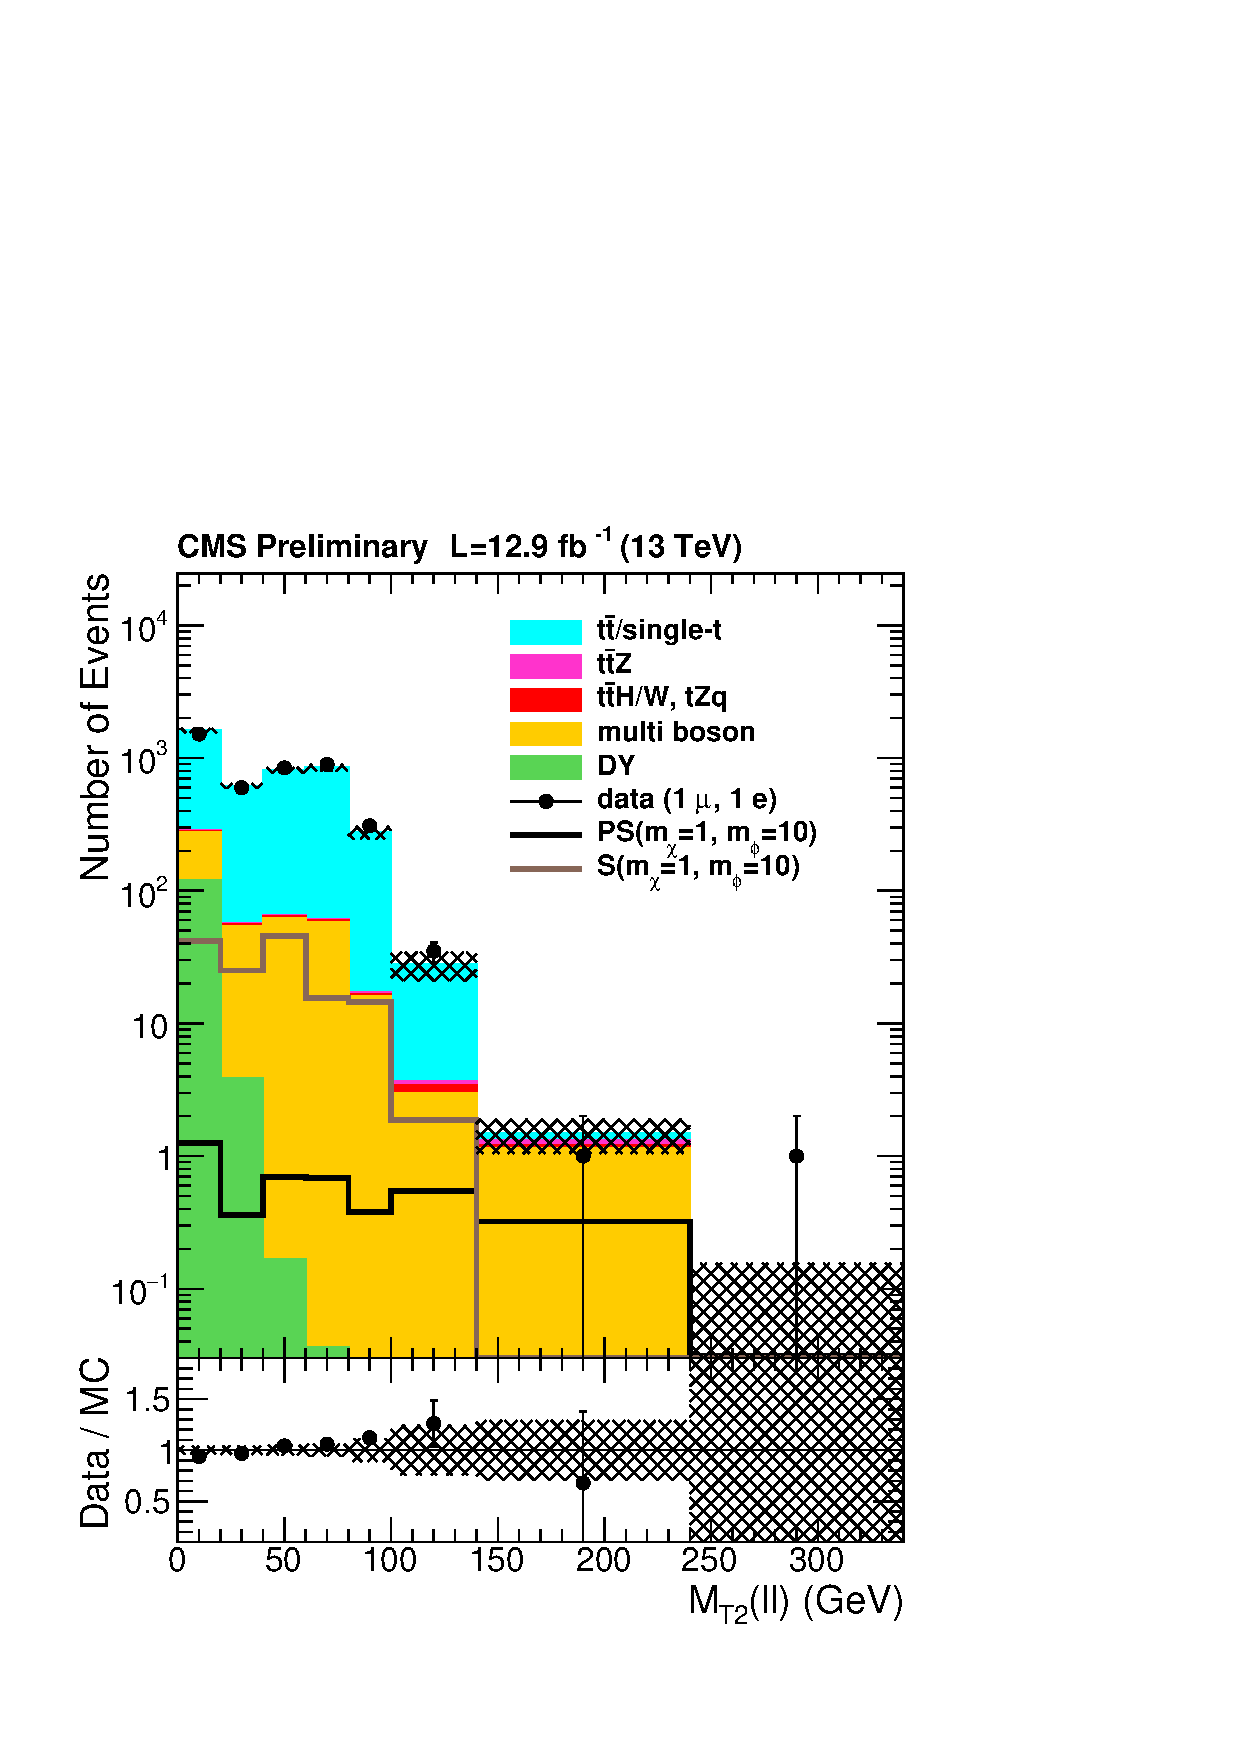
\includegraphics[scale=0.33]{figures/systematicPlots/mue_log_scaled/njet2-btag0-multiIsoWP-looseLeptonVeto-mll20-met80-metSig5/dl_mt2ll.pdf}}\\
\subfloat[ $\Njets \leq 1$, $\Nbtags=0$, low \ETmiss]{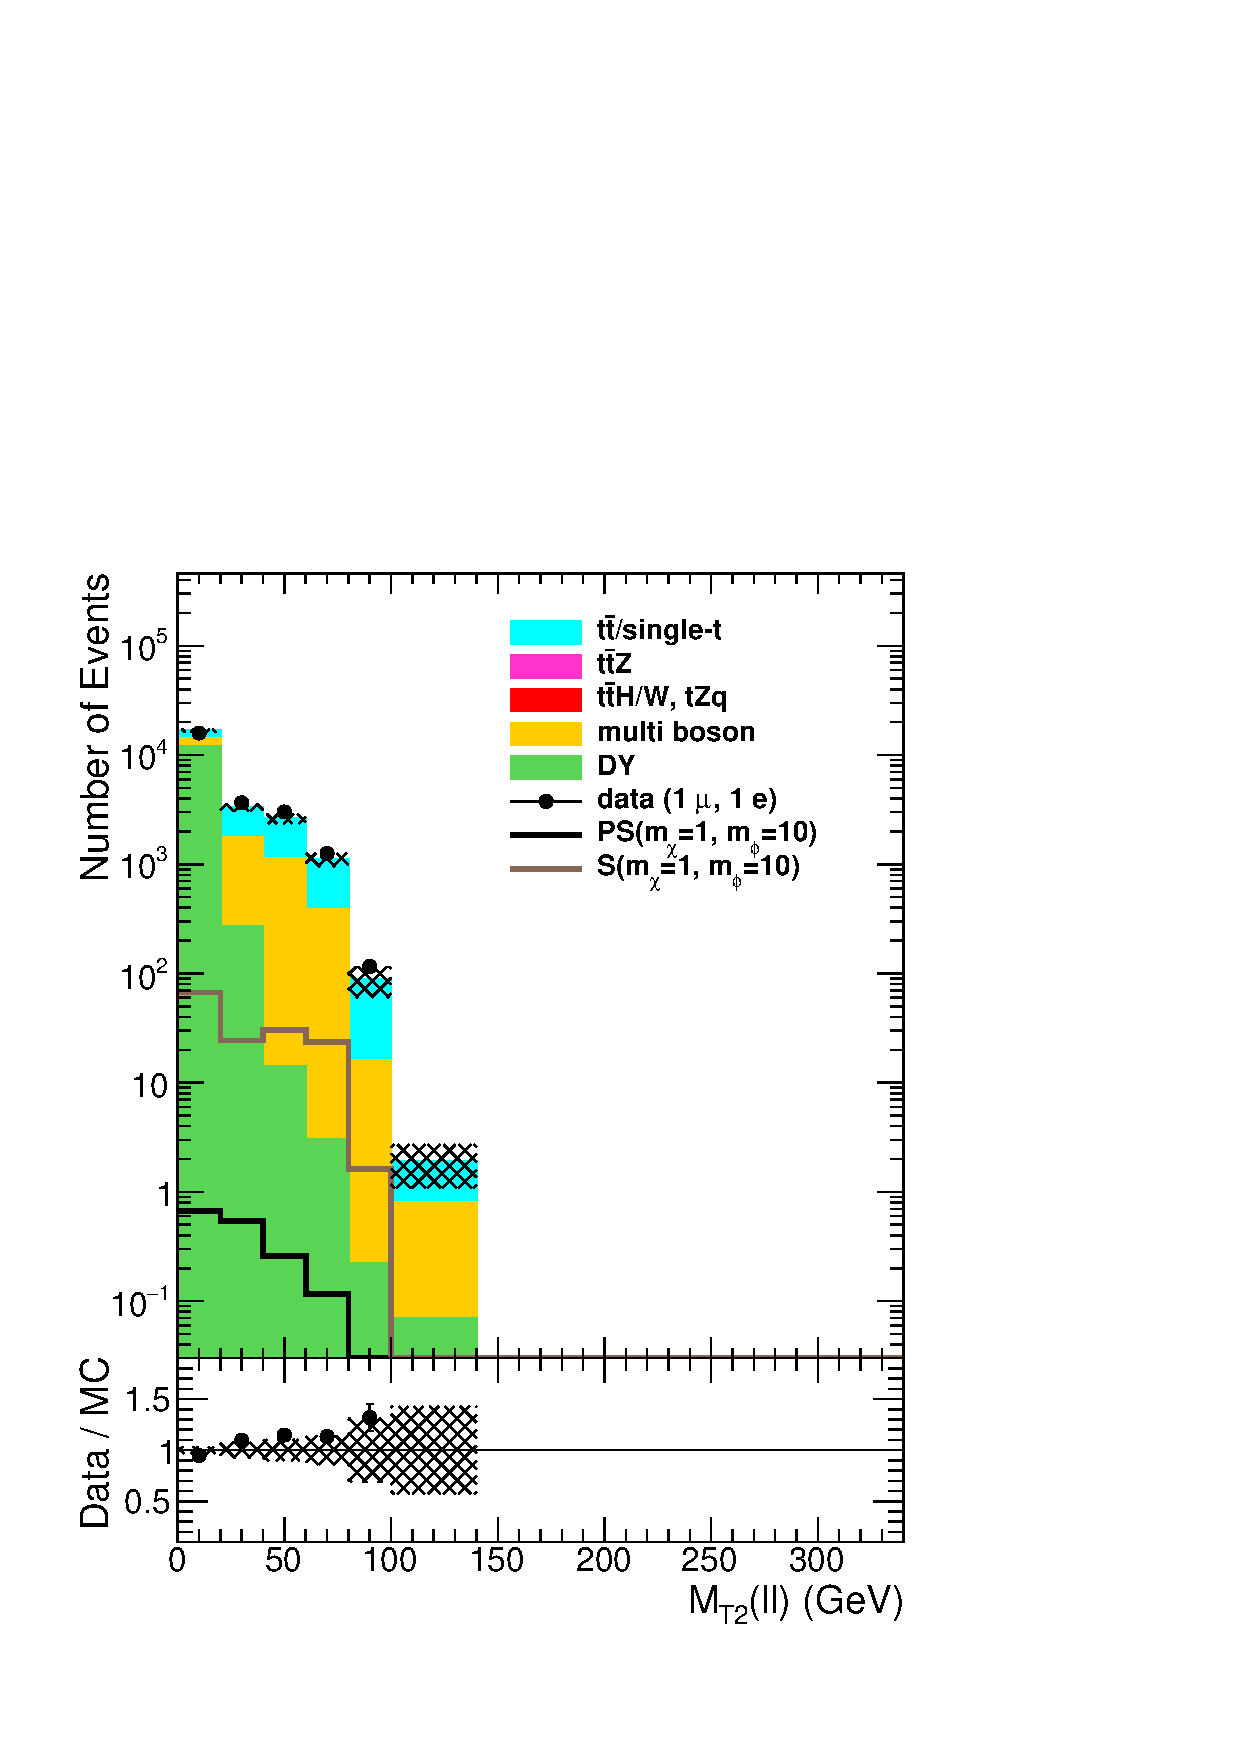
\includegraphics[scale=0.33]{figures/systematicPlots/mue_log_scaled/njet01-btag0-multiIsoWP-looseLeptonVeto-mll20-metInv/dl_mt2ll.pdf}}
\subfloat[ $\Njets \leq 1$, $\Nbtags\geq1$, low \ETmiss]{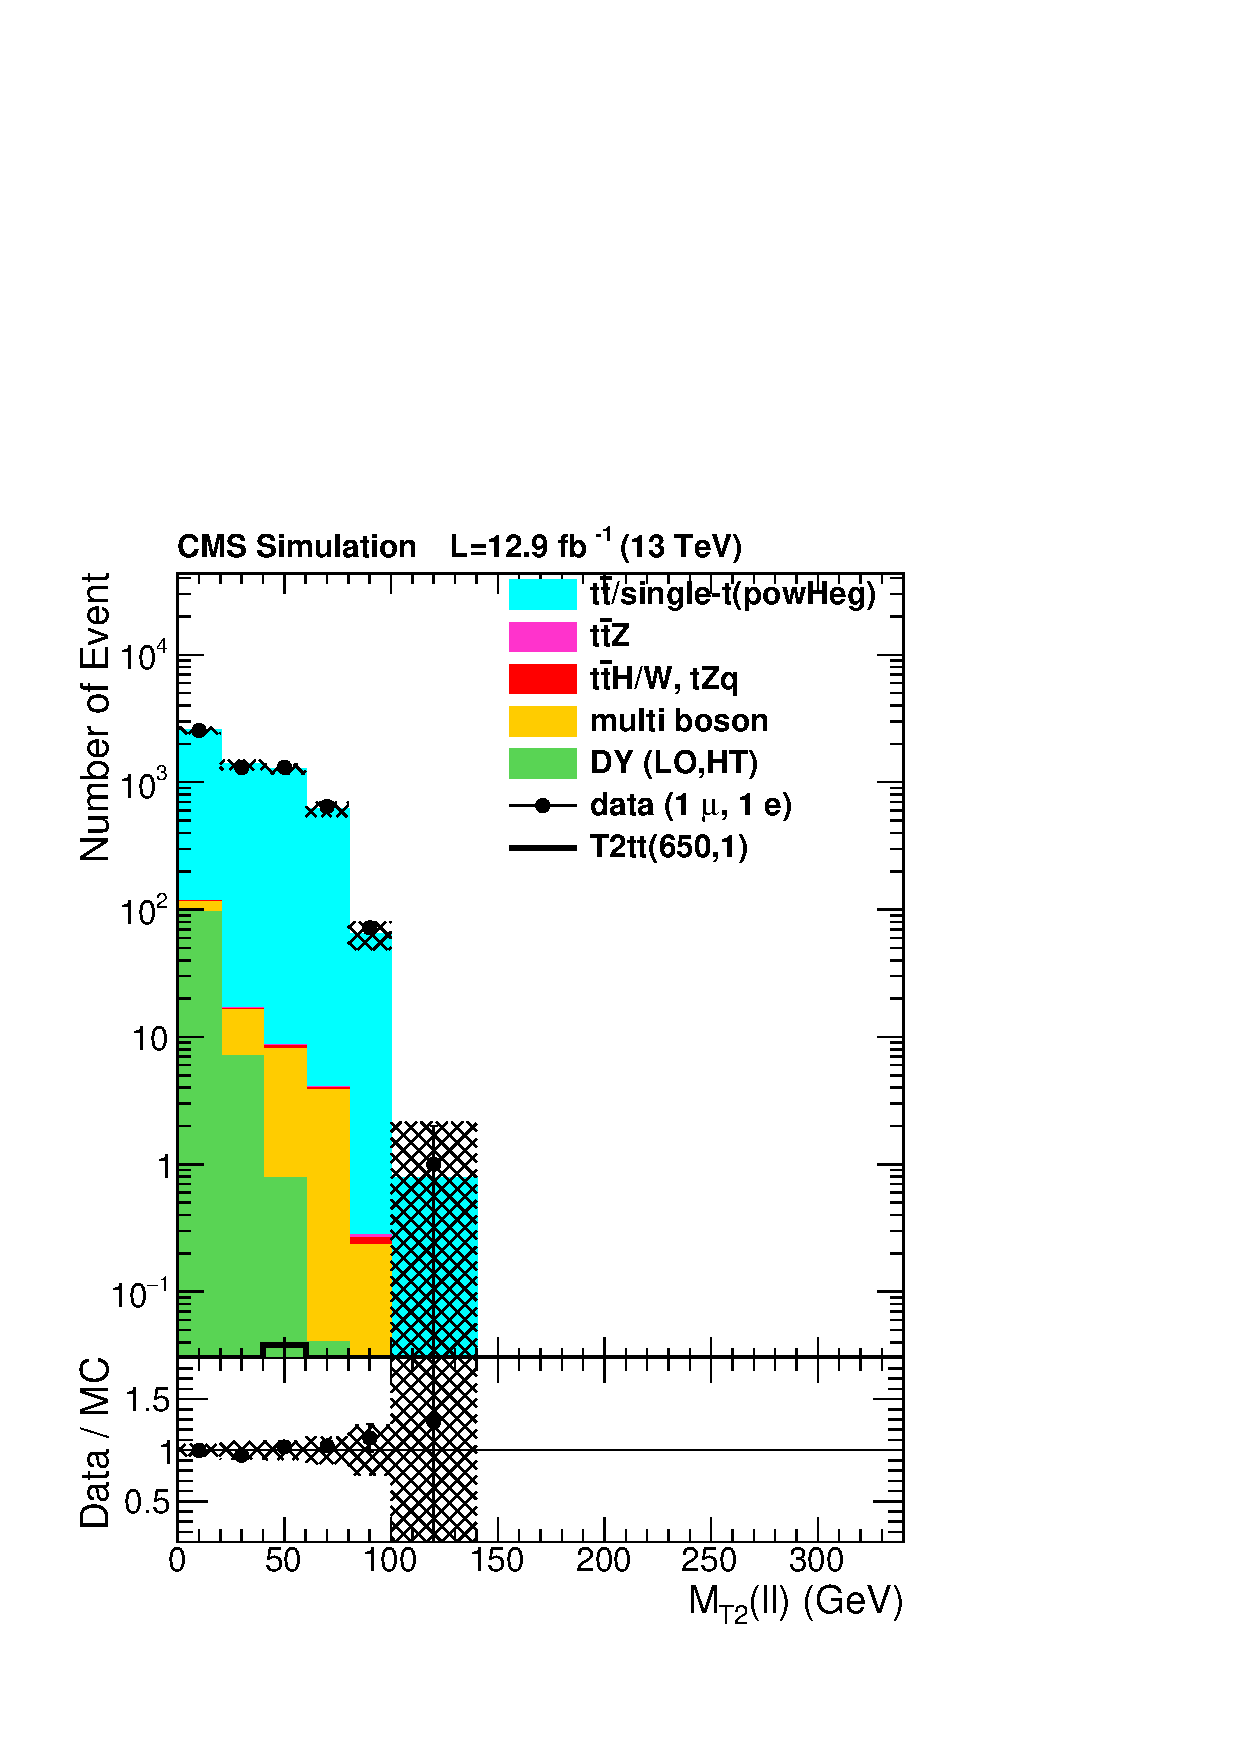
\includegraphics[scale=0.33]{figures/systematicPlots/mue_log_scaled/njet01-btagM-multiIsoWP-looseLeptonVeto-mll20-metInv/dl_mt2ll.pdf}}
\subfloat[ $\Njets \geq 2$, $\Nbtags=0$, low \ETmiss]{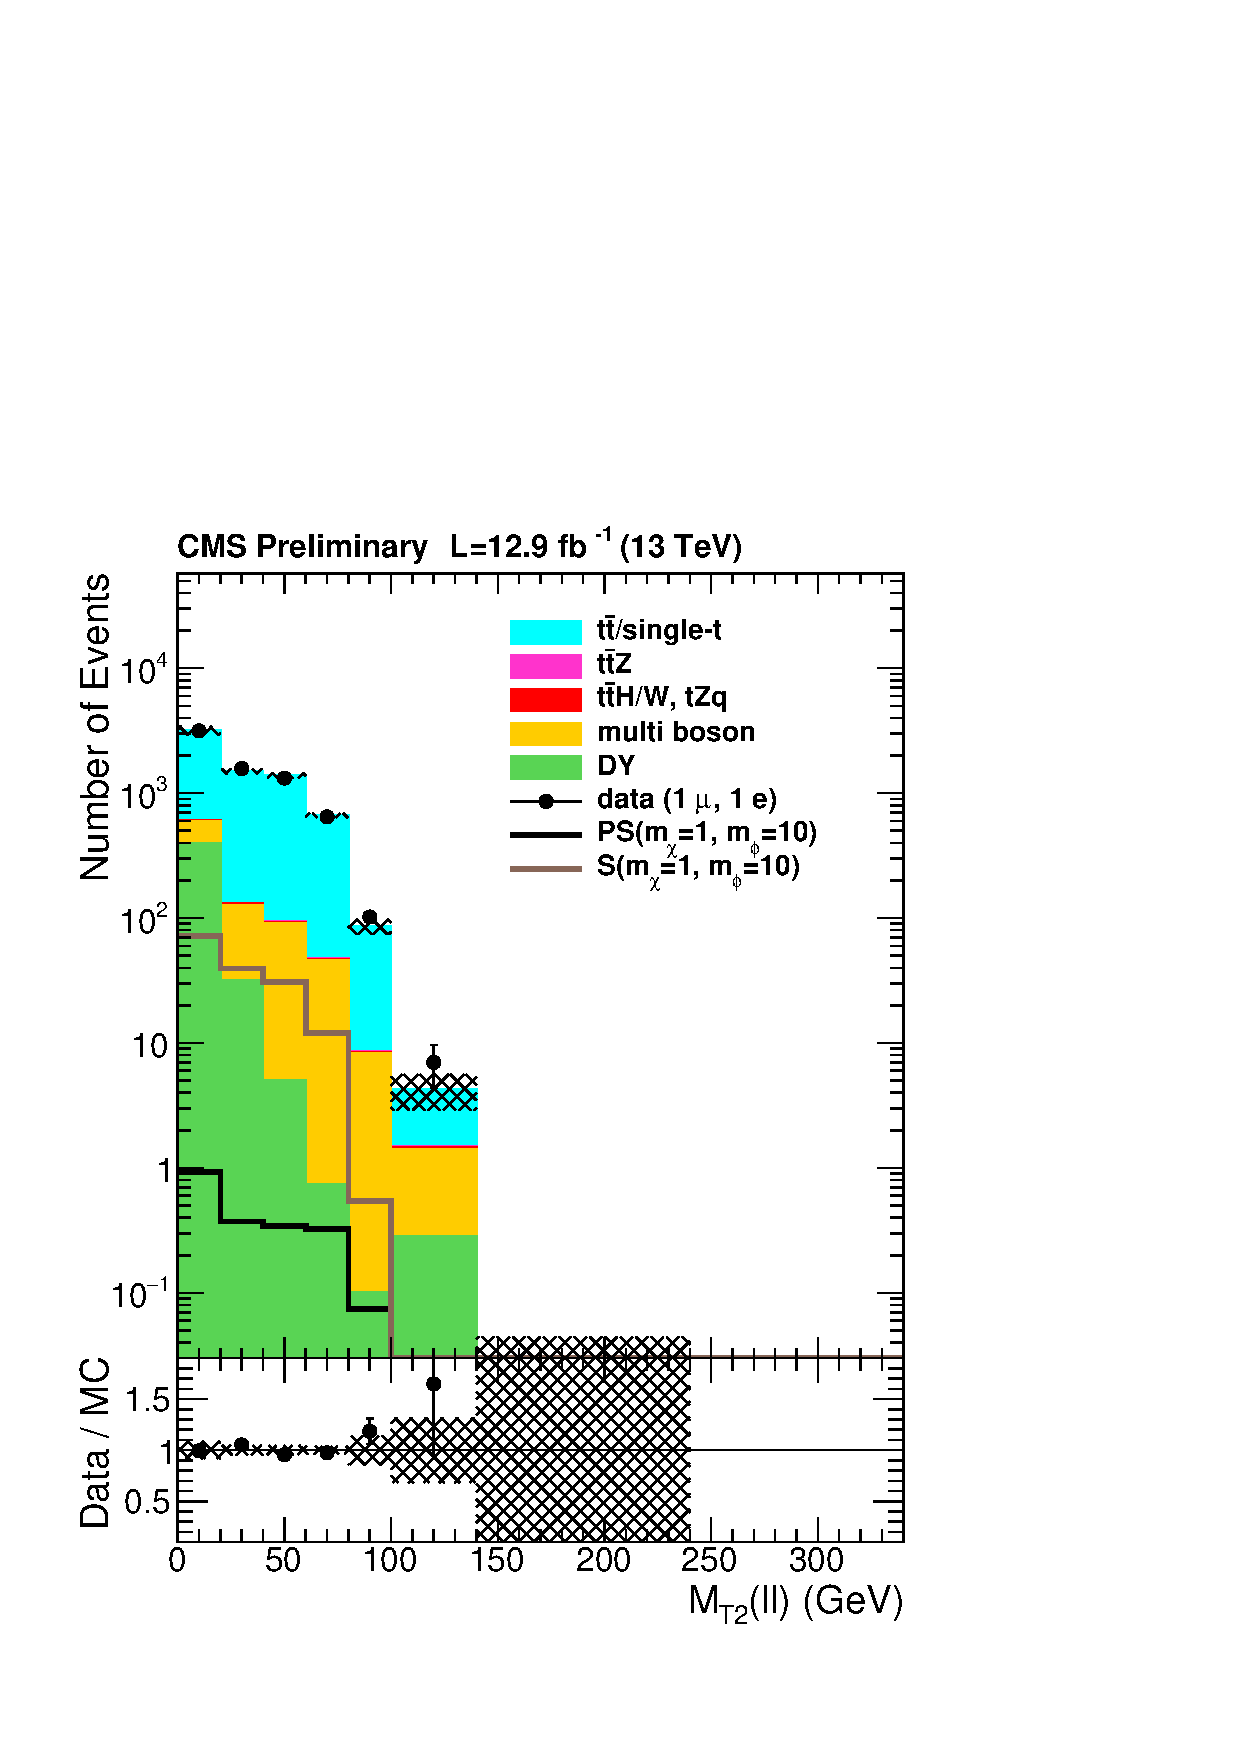
\includegraphics[scale=0.33]{figures/systematicPlots/mue_log_scaled/njet2-btag0-multiIsoWP-looseLeptonVeto-mll20-metInv/dl_mt2ll.pdf}}\\
\subfloat[ $\Njets \geq 2$, $\Nbtags\geq1$, low \ETmiss]{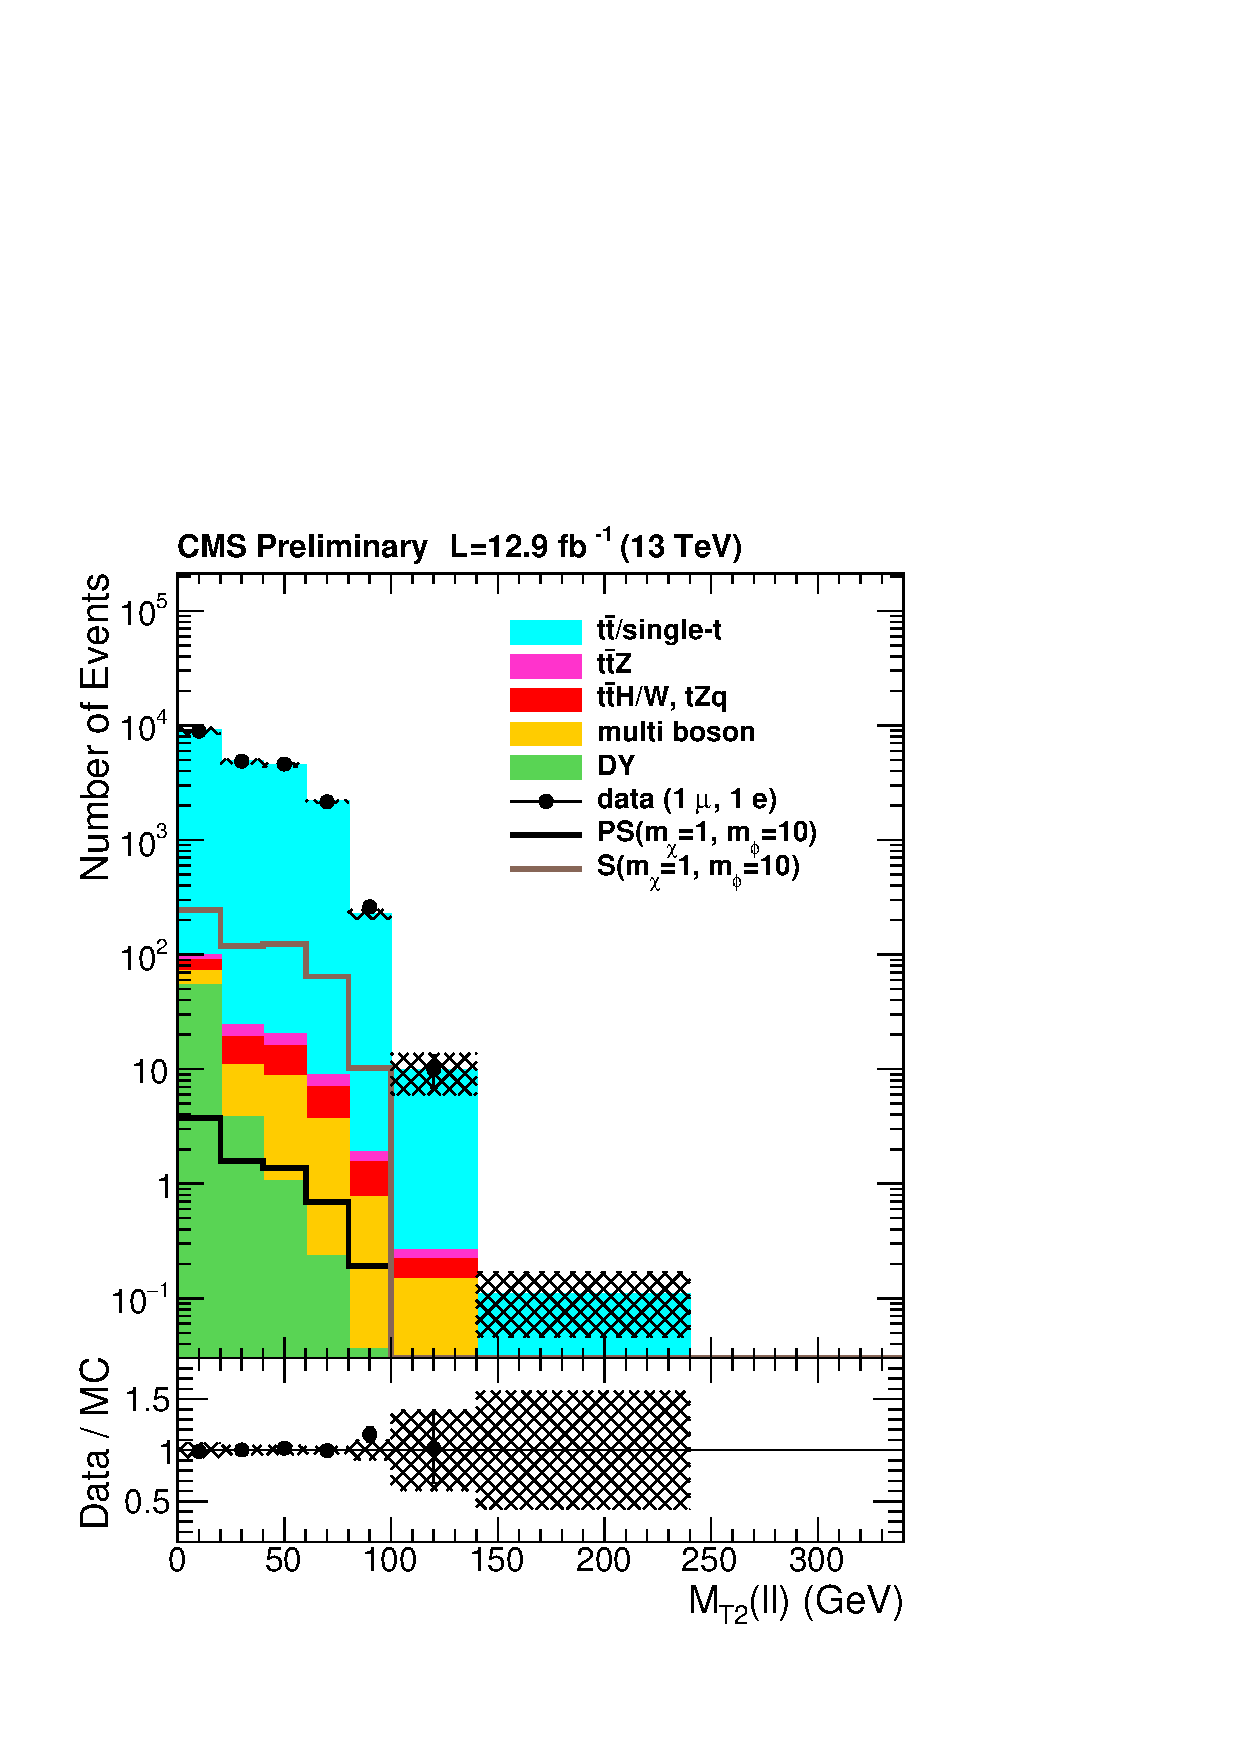
\includegraphics[scale=0.33]{figures/systematicPlots/mue_log_scaled/njet2-btagM-multiIsoWP-looseLeptonVeto-mll20-metInv/dl_mt2ll.pdf}}
\caption{\mtll distributions in opposite flavor control regions enriched by $t\bar{t}$ events. MC yields are normalized to data using the yields at $\mtll<100$ \GeV.  }
\label{fig:ttBar_controlPlots}
\end{figure}

Going beyond the check of the rate of events with large jet mismeasurements in Sec.~\ref{sec:met_tail}, we next check the shape of the \mtll distribution in \ttbar due to \ETmiss mismeasurements and any other potential sources.
In order to remove contamination from DY we require different flavor leptons. 
Figure~\ref{fig:ttBar_controlPlots}  shows the \mtll distribution compared to simulation for various selections. Comparisons are performed in high \ETmiss regions
that are defined by $\ETmiss>80$ \GeV and $\metSig>5$ for different jet and b-tag multiplicities. Of course we omit the signal region by skipping the case $\Njets \geq 2$, $\Nbtags\geq1$.
In the low \ETmiss signal regions given by $\ETmiss<80$ \GeV that case can be included as well. 

We observe a good agreement between \mtll shape from data and simulation over three orders of magnitude change of yields per bin. 
The uncertainty due to experimental effects is shown with a hatched band.

\subsubsection{Summary of \texorpdfstring{\ttbar}{ttbar} background estimation.}

Based on these checks in the control regions we proceed with using MC simulation to predict the top background contribution in the signal regions and we use data events in $\mtll <100$~\GeV for the absolute normalization. 
The normalization is done in each of the channels and yields the following scale factors: $0.867\pm0.010$ in the $\mu\mu$ channel, $0.892\pm0.017$ in the $ee$ channel and $0.861 \pm 0.009$ for $e\mu$ events.
In this way, the experimental uncertainties affecting the overall normalization are largely reduced.
Figure~\ref{fig:ttBar_controlPlots}f shows the side-band with zero b-tagged jets that we use to assign a systematic uncertainty on the \ttbar shape. 
We find 7 events satisfying $\mtll>100$~\GeV and 4.6 events predicted. Despite the fact that statistical uncertainties are large, we apply an uncertainty on the \mtll yield of 50\% for $\mtll<240$~\GeV and 100\% above that threshold.

%Finally, we checked that a veto on hadronically decaying $tau$ leptons does not change the sensitivity of the analysis. 

